\documentclass[../main/main.tex]{subfiles}

\newdate{date}{05}{05}{2020}

\begin{document}

\marginpar{ \textbf{Lecture 15.} \\  \displaydate{date}. \\ Compiled:  \today.}

In the previous lectures, we have presented all the Feymann ruels to write contribution to the perturbative expansion of the Green's function in momentum space.
For example we present the first order contribution to the greeen's function:

it is easy to remember what we have sad, to conclude that these are the two topologically distinct feymann diagrams in momentum space. They correspond to the same topologically distinc diagrams in real space (coordinate space).

The correpsonding analitical expression are the following:

where clearly we have to integrate over the internal wave vectors and remembering that repeated indices must be summed. And for instance concerning the first term we have clearly three non interacting green's function, we have a potential term corresponding to zero momentum (\( U(0) \equiv U (k=0) \)). This is due to the fact that we have to conserve four momentum at each vertex. SO for instance in the graph (a) we have in the first vertex k and k, so the only possibility for momentum is that the q vector is zero!
Of course, we have a closed loop, so we have a minus sign and also an expoential term.
The second term (b) is similar, but here the potential depends on (k-k1) (again we have four momentum conservation at each node) and again we have an expoential factor due to the factor that we have a particle line connected by the same  interaction line. Of course we have again three non-interacting green's function.

We xploit now the fact that actually the non-interacting green's function is diagonal in the spin index, and so we have three deltas, so this means that \(  \lambda=\alpha   \), \(  \lambda' = \beta \) and \( \mu' = \mu  \) in (a). Analogous for  (b) term.
So we can simplify the notation in the second step.


It is clear that the basic topological structure is exactly the same that we have found for the diagrams in coordinate space. However, the labeling and the detailed interpretations are different.

As already sad the term \( U(0) \) is due to the four momentum conservation. Actually (a) correspond to the so called direct term (while (b) is the exchange term) which for instance in the Jellium model is used to cancel is just used to cancel physical divergences.



This is a good point to propose the third homework, which is related to the application of the feymann rules to build the different contribution to the green0s function. We focus on the second order ferymann diagrams. We have already shown them and the first four are these ones. We are invited to write the analitycal expression using the feymann rules which are associated with the first three (a,b,c) diagrams (you have to write integrals with also spin label and so on ) in coordinate space. Then, considering that actually
(c) and (d) diagrams look quite similar, just try to demonstrate that they are really topological distinct diagrams. Finally, just focus on (c) diagram and try to write the analytic expression of (c) diagram, also in momentum space and of course you can either use the feymann rules in momentum space or just take the fourier transform of the (c) contribution in coordinate space.



\section{Dyson's equations}
Why we should introduce such equtions? Because, as we have already seen by mentioning the third homework, even if with the Wick's theorem we can simplify the perturbative expansion and even if with Feymann diagrams you can also simplify the evaluation, because you can really focus on the important physical contact of the different terms, in any case the situation becomes more and more complicated when you consider higher and higher order in the perturbative series. Because, as we have mentioned, for instance already at second order we have 10 topologically distinct diagrams, and one can imagine there is a profilefarition when you increase the order of the perturbative expansion. So clearly, if we want to make a progress and if we want to evaluate a larger number of perturbative terms, we have to introduce some other techniques and tricks to have a further help. These are just represented by Dyson's equations, because thanks to these equations we can summarize Feymann diagrams in a very compact form as we will see.

Now, just as a motivation for introducing such concept, let us come back to the first four second order Feymann diagrams represented in Fig. \ref{fig:15_1}.
Clearly, one can notice, apart from the fact that they are really topologically distinct, but, in any case, it is clear that forgetting the specific and detailed list of labels and writings, that somehow one can construct these four diagrams by combinations of simpler diagrams which are essentially the two topologically distinct first order diagrams in Fig. \ref{fig:15_2}. So even if the four diagrams are topologically distinct, in any case you can clearly think to build them by repetions of these two diagrams.

\begin{figure}[h!]
\centering
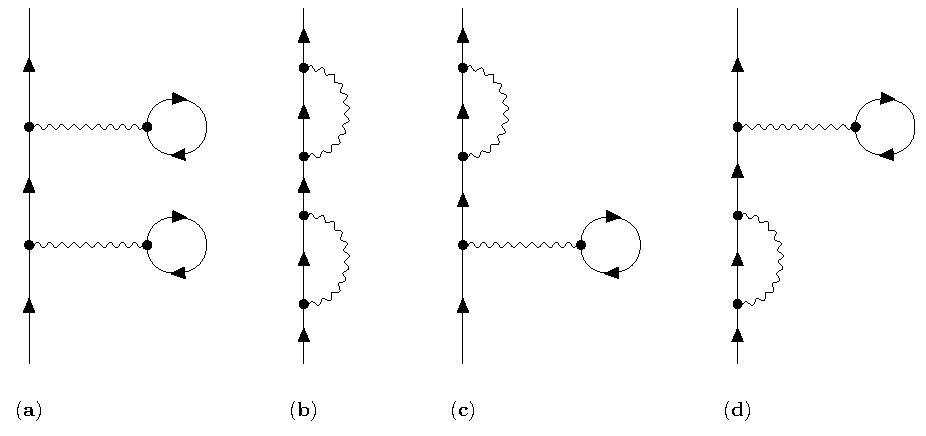
\includegraphics[width=0.9\textwidth]{15_image/tutti.pdf}
\caption{\label{fig:15_1} Four of the 10 topologically distinct connected diagrams at \( 2 \)-nd order perturbative expansion for the Green's function \( G_{\alpha \beta } (x,y) \).}
\end{figure}

\begin{figure}[h!]
\begin{minipage}[c]{0.5\linewidth}
\centering
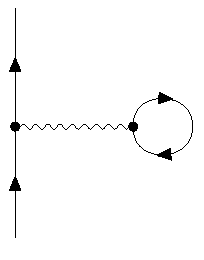
\includegraphics[width=0.5\textwidth]{../lessons/15_image/A.pdf}
\end{minipage}
\begin{minipage}[]{0.5\linewidth}
\centering
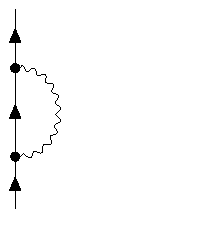
\includegraphics[width=0.5\textwidth]{../lessons/15_image/B.pdf}
\end{minipage}
\caption{\label{fig:15_2} Topologically distinct first order diagrams.}
\end{figure}

This led us to make a first distinction between two kinds of different diagrams:
\begin{itemize}
\item \textbf{improper diagrams}, that can be seprated into two different parts, by cutting a single particle line. This is actually true for all the four diagrams that we have listed above. For instance if we take the (a) diagram of Fig. \ref{fig:15_1} we can separate the diagram into two disconnetted parts by just cutting the central particle line. We obtain two terms like the one of Fig.\ref{fig:15_2}. The same is true for the other three diagrams.

\item \textbf{proper diagrams}, also called “irreducible” diagrams, for which it is not possible to separate them into two parts if you cut just a simple particle line.
For instance, if you come back to the list of ten second order Feymann digrams, the diagram (i) (Fig. \ref{fig:15_3}) cannot be separated into two disconnetted part.

\marginpar{
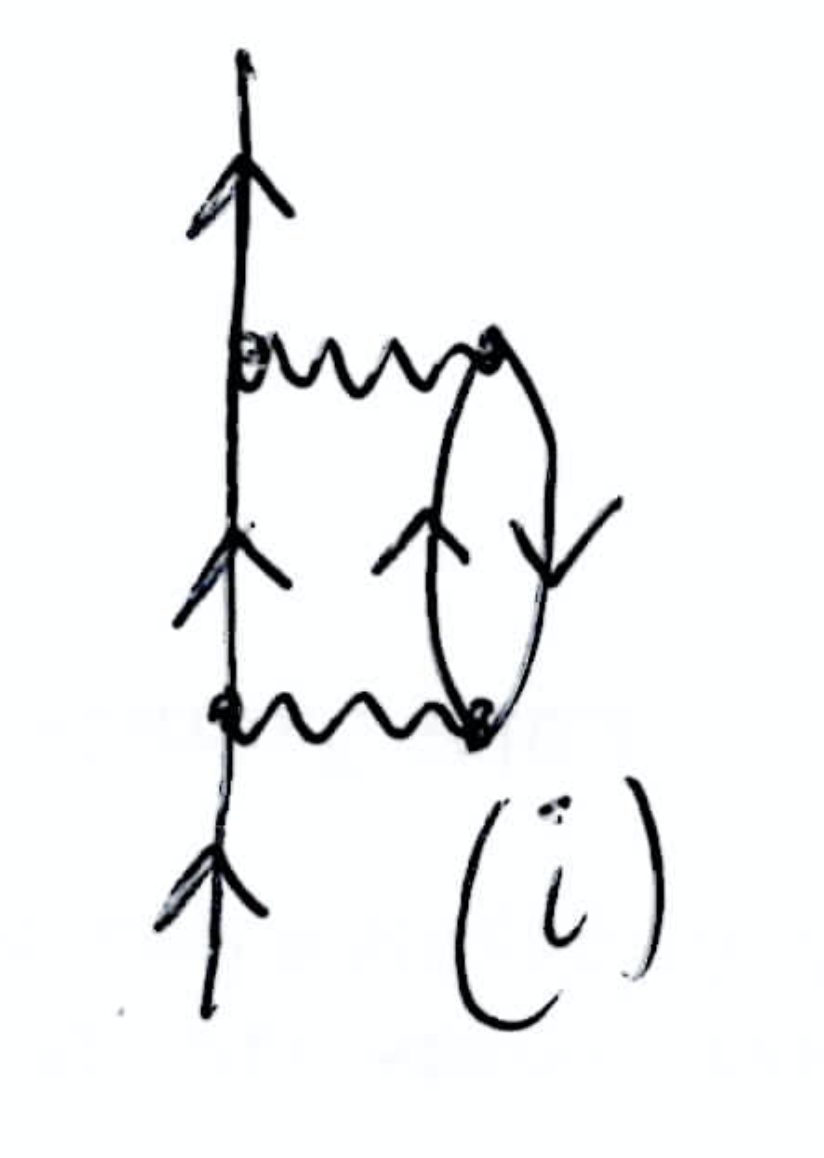
\includegraphics[width=\marginparwidth]{../lessons/15_image/1.png}
\captionof{figure}{\label{fig:15_3} Second order Feymann diagram: (i) diagram.}
}

\end{itemize}

Now, let us come back to the exact full interacting Green's function which can be rewritten as a non-interacting Green's function plus a collection of infinite terms as in Fig. \ref{fig:15_4}. The last have the property of be connected with a free Green's function at each end (at the beginning and at the end). What is in the middle (so, a sum of infinite terms) is what we call a \textbf{self-energy} \( \Sigma  \) and we will see in the future the precise meaning of such a quantity.

\begin{figure}[h!]
\centering
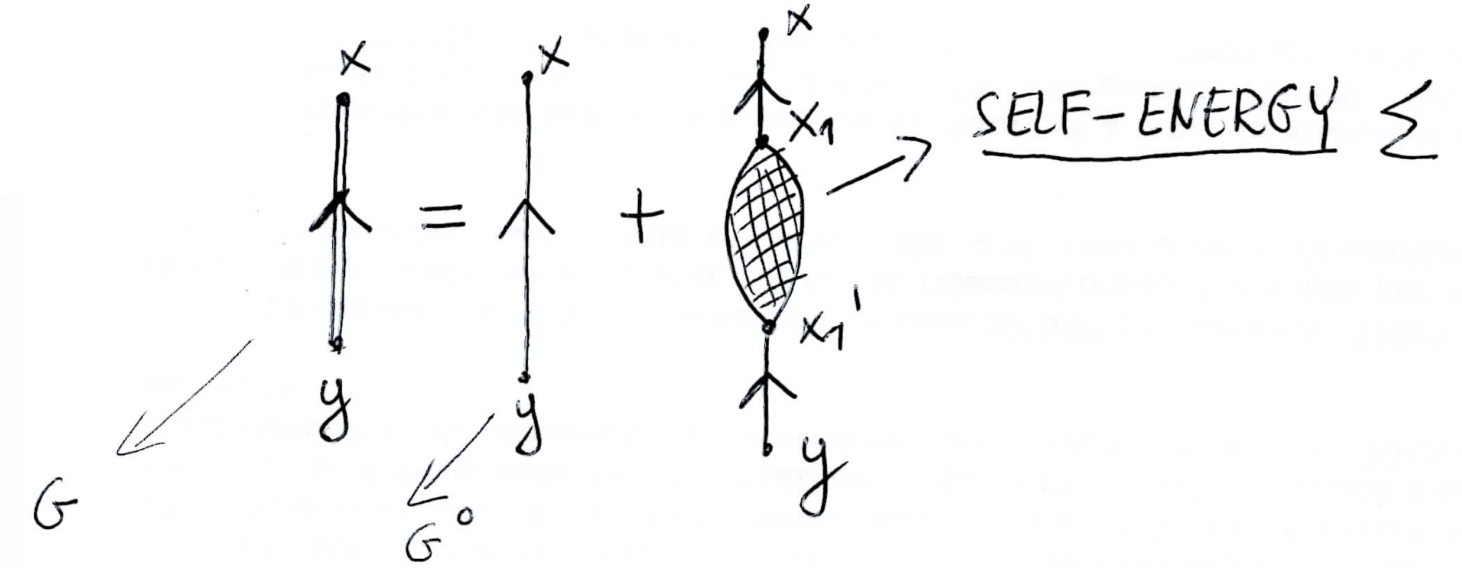
\includegraphics[width=0.8\textwidth]{../lessons/15_image/2.png}
\caption{\label{fig:15_4} Exact Green's function expansion.}
\end{figure}

Clearly, this is just a formal writing that it is realted to the corresponding analityc expression, that clearly can be written in this way:
\begin{equation*}
  G_{\alpha \beta } (x,y) =
  G^0_{\alpha \beta } (x,y)
  + \int_{}^{} \dd[4]{x_1} \int_{}^{} \dd[4]{x_1'}
  G^{0}_{\alpha \lambda } (x,x_1) \Sigma (x_1,x_1')_{\lambda \mu }
  G^0_{\mu \beta } (x_1',y)
\end{equation*}
where the “self-energy” is just the sum of all the so called \textbf{self-energy insertions}, that are any part of the diagram that it is connected to the rest of the diagrams by the two particle lines (one in and one out).
So, clearly if we know \( \Sigma  \) exactly, then in principle we have also the exact Green's function. Hence, we have just shifted the problem of finding the exact Green's function to that of find the exact self energy.

Now, coming back  to the concept of proper and improper diagrams, also for the self-energy and for the self-energy insertions we can define a \textbf{ proper self-energy insertion} as a general  self-energy insertions that has the property that cannot be separated into two disconnetted pieces by cutting a single particle line.  We define the \textbf{proper self-energy} \( \Sigma^*  (x_1,x_1')_{\alpha \beta }\) (just to distinguish it from the self energy \( \Sigma  \)) which is the sum of \emph{all} the proper self-energy insertions.
Clearly, \( \Sigma  \) can be written as a sum of all the possible repetions of the proepr self-energy \( \Sigma ^* \). This is clearly something that you expetced since the proper self-energy contains essentially all the irreducible diagrams. More specifically, the self energy is:
\begin{equation}
\begin{split}
    \Sigma (x_1,x_1') = & \Sigma^* (x_1,x_1')
    + \int_{}^{} \dd[4]{x_2} \int_{}^{} \dd[4]{x_2'} \Sigma^* (x_1,x_2)
    G^0 (x_2,x_2') \Sigma ^* (x_2',x_1')
    \\
    &+ \int_{}^{}  \int_{}^{} \int_{}^{} \int_{}^{} \Sigma ^* G^0 \Sigma ^*  G^0 \Sigma ^* + \dots
\end{split}
\end{equation}
so it is the proper self energy, plus a term where you have two proper self energy connected by a particle line, plus another term with three proper self energy connected by two non-interacting lines and so on and so forth.
In terms of the Feymann diagrams the situation is like in Fig. \ref{fig:15_5}. In particular, we have \( \Sigma  \) which is plotted as a bubble with a double dahsed line which is equal to the proper self energy (a bubble with a single dashed line) plus all the possible repetions of this self energy.

\begin{figure}[h!]
\centering
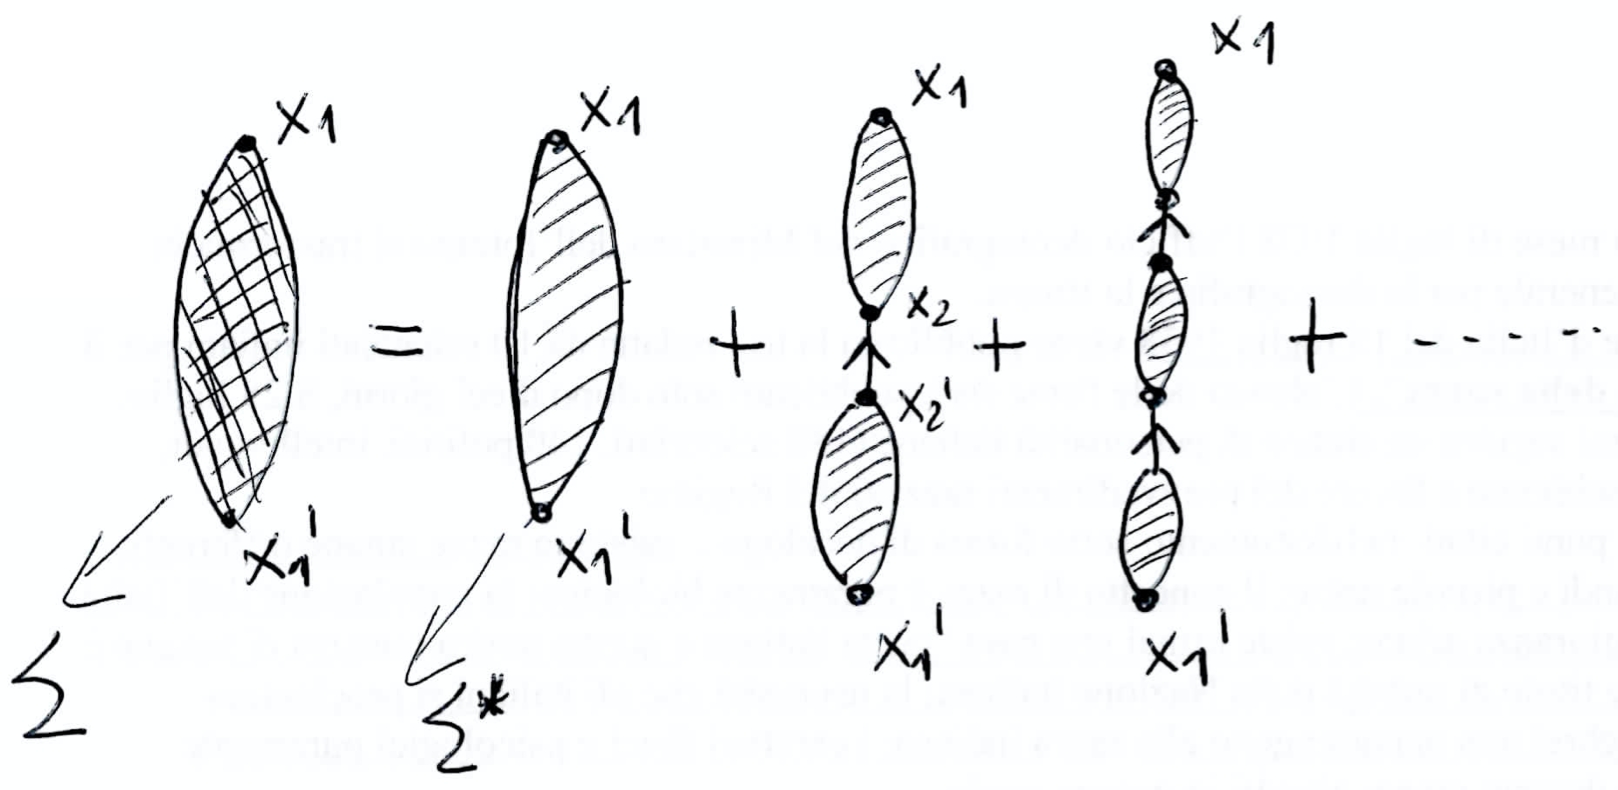
\includegraphics[width=0.7\textwidth]{../lessons/15_image/3.png}
\caption{\label{fig:15_5} Expansion of the self-energy.}
\end{figure}


Now, clearly since, as said, the Green's function can be written as the non-interacting Green's function plus the self-energy connected with single particle lines, we can also rewrite the Green's function in terms of the proper self energy as:
\begin{equation}
\begin{split}
    G(x,y) = & G^0 (x,y)
    + \int_{}^{} \dd[4]{x_1} \int_{}^{} \dd[4]{x_1'} G^0 (x,x_1) \Sigma ^* (x_1,x_1') G^0 (x_1',y) \\
    &+ \int_{}^{} \int_{}^{} \int_{}^{} \int_{}^{} \mathcolorbox{yellow!40}{G^0} \Sigma ^* G^0 \Sigma ^* \mathcolorbox{green!20}{G^0} + \dots
\end{split}
\label{eq:15_1}
\end{equation}
where we the first terms is the non-interacting Green's function, the second term has in the middle the proper self energy, plus all the other possible repetions of the proper self energy with an interacting line in (green term) and an interacting line out (yellow term).
Now, again we have done nothing, because we have just shifted the problem from finding the exact Green's function to that of find the exact proper self-energy.


However, now the trick is the following. Formally, we can rewrite the last expression in a much more compact way in this form:
\begin{equation}
  G_{\alpha \beta } (x,y) = G^0 _{\alpha \beta } (x,y)
  + \int_{}^{} \dd[4]{x_1}  \int_{}^{} \dd[4]{x_1'} G^0_{\alpha \lambda } (x,x_1) \Sigma ^* (x_1,x_1')_{\lambda  \mu } \mathcolorbox{green!20}{G_{\mu \beta } (x_1',y)}
  \label{eq:15_2}
\end{equation}
which is called the \textbf{integral Dyson's equation}. Essentially, the structure is exactly the same of the previous equation, but with the difference that at the end we have, in place of the final non-interacting Green's function, the exact one. So, the exact Green's function is present both in the right hand and on the left hand of the equation.
Since this is the quantity we want to compute, we have a complicated integral equation. Of course we can easily verify this equation by just iterating the right side. For instance, if we simply replace \( G \) with  \( G^0 \) we find the first term, if then we put inside the \(G\) the first order correction, we get the second order correction and so on and so forth.

To reasume, the last equation is much more compact and the same is true for the corresponding diagrams illustrated in Fig. \ref{fig:15_6}. In particular, the first expansion in this figure is the graphical representation of Eq. \eqref{eq:15_1}, while the second one of Eq. \eqref{eq:15_2}. Here, the full-interacting Green's function is represented with a double arrow as on the left hand side.

\begin{figure}[h!]
\centering
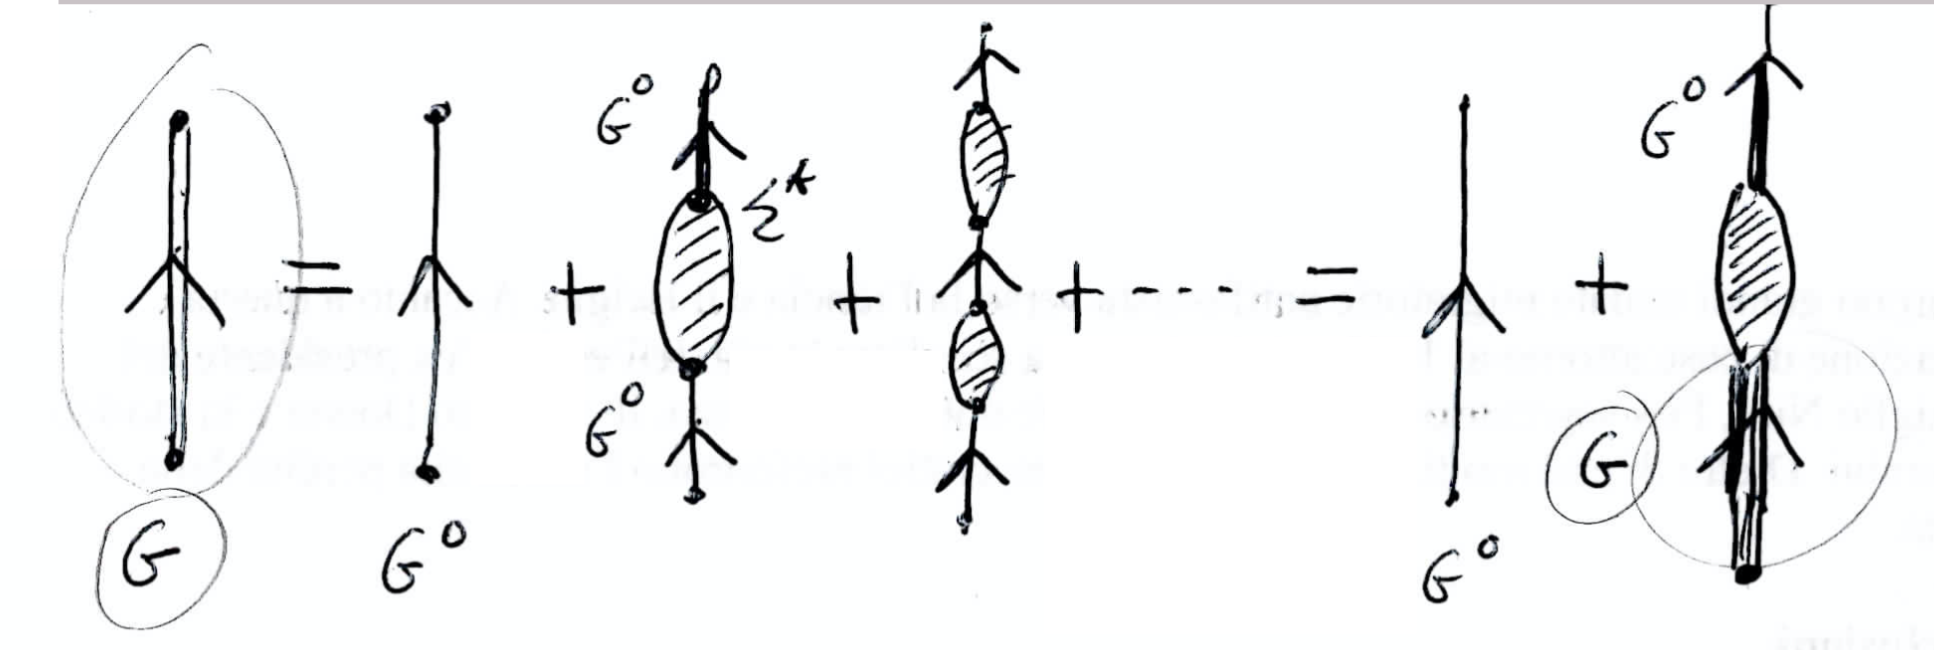
\includegraphics[width=0.7\textwidth]{../lessons/15_image/4.png}
\caption{\label{fig:15_6} Expansion of the Green's function. The first expansion is the graphical representation of Eq. \eqref{eq:15_1}, while the second one of Eq. \eqref{eq:15_2}.}
\end{figure}

To summarize, we repeat that we have just reduced the problem of evaluating the exact Green's function to that of evaluating the exact proper self-energy \( \Sigma ^* \).
For a non uniform system, the integral Dyson's equation, that in principle can be solved by iteration, is indeed a very complicated equation. But, as we see in a while, actually the Dyson's equation becomes much simpler in the case of a uniform system.

\section{Dyson's equation for uniform systems}
The integral Dyson's equation in real space is a complicated equation.
The idea is that the situation becomes much simpler for uniform systems, which are translationally invariant systems. The point is that the Dyson's equations becomes an algebraic equation, instead of an integral equation.

The idea is that for such a uniform system all the relevant quantity \( G,G^0, \Sigma , \Sigma ^* \) depend only on the coordinate differences and so we can introduce 4-dimensional Fourier transforms. For instance, one can write the proper self energy (which now just depends on the difference between the coordinates) in this way:
\begin{equation*}
  \Sigma ^* (x,y)_{\alpha \beta } = \Sigma ^* _{\alpha \beta } (x-y)
  = \frac{1}{(2 \pi )^4} \int_{}^{} \dd[4]{k} e^{i k (x-y)} \mathcolorbox{green!20}{\Sigma ^*_{\alpha \beta } (k) }
\end{equation*}
where \( \Sigma _{\alpha \beta }^* (k) \) has the meaning of the Fourier transform of the proper self energy.

Now, it is very easy to demonstrate (we do not do it explicitly, we have just to replace all the quantities in the integral Dyson's equation \eqref{eq:15_2}, by the corresponding Fourier expansion), that we arrive at the \textbf{algebraic Dyson's equation} in momentum space:
\begin{equation*}
  G_{\alpha \beta } (k) = G_{\alpha \beta }^0 (k) + G_{\alpha \lambda }^0 (k) \Sigma ^* (k)_{\lambda \mu } G_{\mu \beta } (k)
\end{equation*}





minute 2:06

















where again we have the exact green's function on the left and right hand side. Clearly a complication remains because this is a complicated equation due to all these spin indices. But the situation becomes even simpler if (as it is often the case) these quantities are also diagonal in the matrix indices. For instance the green's function can be written as \( G_{\alpha \beta } = \sigma _{\alpha \beta } G\). Now if this is the case, the situation is very very simpler, because at that point we can write an explicit expression for the exact green's function:
..
(obtained by multiplying and dividing for the non-interacting green's function).

What is the meaning of the quantity \( [G^0(k)]^{-1} \)? This is the inverse of the non-interacting green's function and remeber that the non-interacting green's function can be written as:
..
Let us remember that in the derivation, the crucial role played by these imaginary quantity \( \eta  \) was related to the fact that of course when these denominators are closed to zero you have a larger contribution to the function so these factors are very important. Instead, if you use the inverse of the green's function, these imaginary small corrections are no longer relevant and you can easily write that the inverse of the non-interacting green's function is simply such a quantity:
..
where we remember that \( \omega _k \) is the non-interacting  single particle energy a part of a \( \hbar  \) factor.

So clearly, we can write explictly the exact interacting green's function in this way:
..
and if we compare this expression with essentially the non-interacting one, we notice that we have a similar form but with the difference that the energy is no longer, as in the non-interacting case, given by the nnon-interacting energy but you have a correction which is just given by the proper self energy. SO if you want the proper self energy plays the role of an additive correction, called additive renormalization, of the non-interacting energy.

Of course we cannot say that we have the explicit form of the exact green's function because of course the problem is just shifted to that of finding the \( \Sigma ^* \). However the real power of the dyson's equation is that if you have any approximation (of course we have forced to have approximation for this \( \Sigma ^* \) but just for a single term of \( \Sigma ^* \), we get automatically an infinite order approximate series for the green's function. Because remember that actually this dyson's eqaution was a more compact way to keep track of all the possible infinite terms. So clearly if you have an approximation for the \( \Sigma ^* \), of course you do not have the exact green's function but you have in any case an infinite order series for the green's function that is really written in a compact form.


If you want you can see it as considering the analogy with the geometrical series. You can remember if you have an infinite sum like this, if \( \abs{x}<1  \), this can be written as \( 1/(1-x) \) (a very easy and compact result).

So we have achived a very important result, because at least we have the formalism (the tools) to really take into account infinite terms in the perturbative approach for the green's function and so for every important quantity in our system. Of course it does not  mean that we have the exact solution but at least we have an infinite number of terms.


Now we can also observe another thing, of course \( \Sigma ^* \) is in general a complex quantity (a complex function) so it has a real and imaginary part.
Now let us remember the Lehmann representation that it is a formal expression for the general exact interacting green's function. SO a part from details, the basis structure of such a green's function in the lehmann representation was a sum of two contributions:
..
let us remember that essentially the first term corresponds to poles just belowe the real axis of the frequency on the right with respect the chemical potential divided by hbar, while the second term corresponds to the present of poles slighlty above the real axis on the right with respect to the chemical potential. Now if you compare this structure with the dyson equation found above (pagina 9!!! \( G_{\alpha \beta } (k) \) la chiamo IMP1), but considering that the \( \Sigma ^* \) in general has an imaginary contribution, now is clear that we have such a relations:
\begin{equation*}
  \begin{cases}
   \Im \Sigma ^* (\va{k},\omega ) \ge 0 & \text{for } \omega < \mu /\hbar \\
   \Im \Sigma ^* (\va{k},\omega ) \le 0 & \text{for } \omega > \mu /\hbar
  \end{cases}
\end{equation*}
of course for the first case it means that, since in the equation IMP1 we have the minus, we are in a situation like for the second term of the green's function given in lehmann representation that gives a pole \( \omega _{pole}=... \), so this is true for frequency \( \omega < \mu /\hbar  \).
Instead for the second case we are in the case of the first term (for the minus sign we have a plus sign) so this is true for frequency \( \omega > \mu /\hbar  \).

This means that clearluy the chemical potential of a system can be determined as the point where the imaginary part of the proper self energy changes sign. So if you know this proper self energy you also know essentially the position (for instance by changing the frequency) of the chemical potential.

Now, we have sad that in any case for any approximation for \( \Sigma ^* \)
this leds to an infinite approximate series in the perturbative expansion.

For instance the simplest possibility is just to use the first order approximation for the  self energy. SO remember that we have seen that the proper self energy for the first order contribution is just given by the sum of those two diagrams:
..
where the arrows just specify how to connect these diagrams to the incoming and outcoming non-interacting green's function.
Now clearly, for this first order terms (essentially both the two diagrams are irreducible, so they are proper diagrams). It means that essentially in this simple case the proper self energy coincides with the self energy and so the proper self energy at first order is just given by those two terms.
Of course a part from the different labelings of the different points, the topological form is the same both in coordinate space and in momentum space.

Now, let us suppose to use in the dyson equation as an approximation of the proper self energy, just the sum of these two terms, and so if we choose such simple approximation \( \sigma ^* \simeq \Sigma ^*_{(1)} \), we get the following approximate green0s function (which of course is an expnasion with infinite term).
So we repeat: even if we consider just a couple of terms (diagrams) we ends up with an infinite series:
...
but of course it does not mean that the resulting green's function is exact, because of course we have an infinite number of terms but they are just obtained by repeating all the possible repetitions of those two fragments.

So this is a very important achivement because let us say, even for very low approximation for \( \Sigma ^* \) we get an infinite series.


Now the interesting result is that essentially we speak about dyson equation, because actually what we have shown for the green's function can be extended to other interesting functions. For instance we can write dyson equation also for the interaction between particles. Of course we have seen that basically the our diagrams are made by two ingredients: we have the green's function (the lines) but also we have the interaction lines (waving lines).

Now it is easy to show that also for the interaction between particles, we can write a dyson like equation. Why?
Let us consider the following formal graphical expression, because it is easier to consider than the analitical expression:
..
we can write the so called renormalized (or dressed) interaction (physically it means essentially the interaction modified by the presence of the medium, so the presence of the interacting particles) as the sum of the \emph{bare interaction} (for instance the bare coulomb interaction) plus something else, where something else is made by an interaction line incoming and an interaction line outcoming and something in the middle (which of course is the sum of all the connected diagrams that are linked by two, incoming and outcoming, interaction line). To what is in the middle we give the name of \textbf{polarization} (the meaning will be clear in a while).

Of course this corresponds to a complicated integral equation, but again as we have shown for the green's function, for a uniform system the equation is much simpler in momentum space. Even in this case we skip the steps to derive this equation because they are trivial, and we arrive at the following formula:
..
where essentially we have that the dressed interaction is given by the bear interaction plus the second quantity with the polarization in the middle. Clearly it is similar to what we have done with self energy and green's function.

Now again by following the same approach we can introduce a new concept, the one of \textbf{proper polarization} which is named \( \pi ^* \). What is the meaning of the proper polarization?
Essentially we define a proper polarization insertion as a polarization part that cannot be separated into two polarization parts just by cutting a single interaction line (this is exactly the same definition of the self energy, the only difference is that while in that case the problem was the ability to cut a single \emph{particle}  line in such a way to have disconnetted diagrams, in this case you are checking wheter it is possible to separate the diagrams into two disconnetded part just by cutting a single \emph{interaction}  line).

These are just two examples:
..
where the first is clearly an improper diagram, because you can easily disconnect the diagrams into two fragments just by cutting a single interaction line, while the second is a proper polarization insertion because this is not possible.

Now this allows us as for the self energy to write a corresponding dyson equation for \( U \) that in momentum space becomes essentially an algebraic equation:
..
So we can write that \( U \) is the bear interaction plus the bear interaction multiplied by the proper polarization and finally by the dressed interaction. So clearly the unknown quantity that we want to compute is present both on the left hand and on the right hand of the equation. Clearly the corresponding graphical representation is the following:

where on the left we have a double waving line, which represent the dressing interaction, then we have the bear interaction and then we have the bear interaction multiplied by proper polarization and at the end again we have the dressed interaction (double waving line).
I have indicated with a single dashed region the proper polarization to be distinguished by the polarization drawn above (with the double dashed region).

This as we will see is a very important achievement because we can really arrive at the form for the dress interaction which is very meaningful for a physical point of view.




\end{document}
